\section{Background}
\subsection{Definición de Metales Pesados}
En la industria, los metales pesados se utilizan en una variedad de procesos, desde la manufactura hasta la minería. Sin embargo, la manipulación y control de estos metales presentan serios riesgos para la salud y el medio ambiente. Los metales pesados, incluso en concentraciones bajas, pueden ser tóxicos y perjudiciales. La exposición a estos metales puede llevar a problemas de salud graves, dependiendo de la concentración y la duración de la exposición. Los efectos adversos pueden incluir daño a los sistemas respiratorio, nervioso y cardiovascular, y en casos extremos, la muerte.\\

Los metales pesados considerados en el presente trabajo son:
\begin{enumerate}
    \item \textbf{Plomo (Pb)}: Un metal pesado utilizado en baterías y soldaduras, la exposición prolongada puede causar daños en los riñones, sistema nervioso central, y problemas cardiovasculares \cite{matthews2019}.
    \item \textbf{Mercurio (Hg)}: Se utiliza en la minería y en algunos procesos industriales, la exposición al mercurio puede causar daño neurológico, problemas renales y efectos adversos en el desarrollo \cite{rao2020}.
    \item \textbf{Cadmio (Cd)}: Se emplea en baterías recargables y en la industria de recubrimientos, la exposición al cadmio puede causar enfermedad pulmonar, daño renal y cáncer de pulmón \cite{nguyen2022}.
    \item \textbf{Arsénico (As)}: Utilizado en pesticidas y en la industria del vidrio, la exposición al arsénico puede resultar en cáncer de piel, enfermedad cardiovascular y daño neurológico \cite{smith2021}.
    \item \textbf{Cromo (Cr)}: Empleado en la producción de acero inoxidable y en tratamientos de cuero, el cromo hexavalente es carcinogénico y puede causar daño a los pulmones y problemas gastrointestinales \cite{johnson2023}.
\end{enumerate}

\subsection{Límites de Concentración y Estándares para Metales Pesados en el Agua}

El monitoreo de la calidad del agua en lo que respecta a la presencia de metales pesados, como el mercurio, el plomo, el cadmio y el arsénico, es fundamental para prevenir riesgos a la salud humana. Las normativas establecidas por organizaciones internacionales, como la Organización Mundial de la Salud (OMS) y diversas agencias regulatorias locales, proporcionan los límites de concentración permitidos de estos metales en el agua potable \cite{truque2006, torres2015}.\\

El sistema de detección propuesto está diseñado para detectar y cuantificar las concentraciones de estos metales, permitiendo activar alertas cuando los niveles exceden los valores permitidos por las normativas vigentes \cite{ding2021, matthews2019}. Estos valores, que se presentan en la Figura 1, son fundamentales para calibrar el sistema y asegurar su precisión y confiabilidad.

\newpage


\begin{figure}[h]
    \centering
    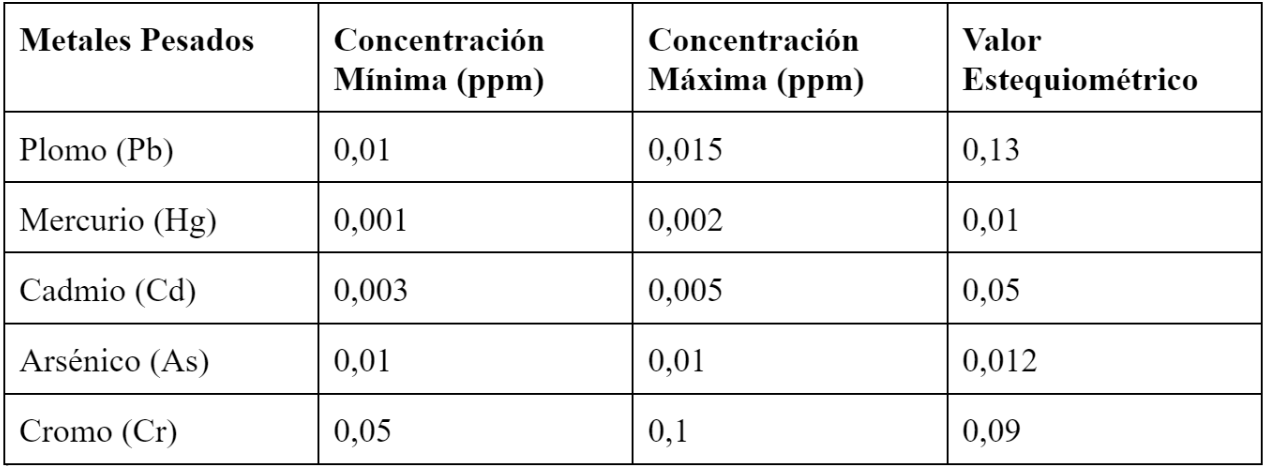
\includegraphics[width=0.5\textwidth]{Recursos/tabla_valores_max.png}
    \caption{Concentraciones permitidas de metales pesados en el agua y valores estequiométricos \cite{truque2006, smith2021, nguyen2022, johnson2023}}
\end{figure}

En la tabla presentan los valores máximos permitidos de concentración para metales pesados como el plomo, el mercurio, el arsénico y el cadmio, los cuales han sido objeto de estudios debido a su toxicidad y efectos adversos para la salud \cite{rao2020, smith2021, nguyen2022}. Estos valores sirven como referencia para el diseño del sistema de detección de metales pesados en el agua, asegurando que las mediciones que realice el sistema cumplan con los requisitos internacionales \cite{johnson2023}.\\

Además, la implementación de este sistema sigue un enfoque de especificación formal para garantizar su robustez y validación. El uso de técnicas formales, como el método Z y otras herramientas de modelado de sistemas, permite describir con precisión el comportamiento del sistema y realizar pruebas exhaustivas para su validación \cite{fitzgerald2009, woodcock1996}.
